\chapter{Evaluación y resultados}
\label{cap:Evaluación y resultados}

Al finalizar el desarrollo se quiso evaluar la visión de los usuarios frente al sistema.
Asimismo, también se pretendió evaluar como de efectivo era realmente dicho sistema,
si de verdad daba resultados su uso o no. Para ello se pidió opinión a expertos en la materia
para que indicaran referencias sobre el sistema, de una forma mas directa. También se hizo
una encuesta de opinión general, rápida y sencilla de responder. Para comprobar su efectividad
se hicieron diversas pruebas de campo. Todo esto está explicado a continuación.


\section{Opiniones de los expertos}

En este capítulo se hablará sobre la evaluación del sistema y los resultados que se obtuvieron.
Para ello se hicieron diferentes pruebas. Recordar que los casos han sido validados mediante
test y estudiados con el experto que nos ayudó a obtener conocimiento sobre el tema.
La primera de ellas fue una evaluación con diferentes
expertos en la materia. Dichos expertos son tanto maestros de salas de armas como tiradores
de alta competición a nivel nacional. No todos dieron permiso para que su nombre saliera, por
lo que se decidió mantener el anonimato de todos ellos para evitar posibles descartes y relaciones.
A cada uno de ellos se les dio acceso a la herramienta para que pudieran probarla y dar feedback
después sobre la misma.

A continuación se puede ver un resumen de las evaluaciones de los expertos consultados:
\begin{itemize}
  \item \textbf{Experto 1:} Este experto es un tirador. Comenta que la idea es buena, el cuando ayuda
    a sus compañeros novatos le comenta el porqué de las cosas para que puedan comprenderlas. Es por esto
    que dice que es buena idea, pero que de momento de queda corta.
  \item \textbf{Experto 2:} Entrenador de alta edad. Comenta que él cuando comenzó apenas había documentación
    sobre el tema, ahora los jóvenes pueden buscar diferentes referencias donde encontrar información
    o incluso en las competiciones preguntar, pero que en sus tiempos nadie te decía nada si no eras de su club.
  \item \textbf{Experto 3:} Tirador de alta edad. Comenta que no es para nada útil. El no confía en una herramienta
    de este estilo, no por ser tecnológica, sino porque cree que no hay un árbol táctico en esgrima. El piensa que
    cada situación es única y no se puede aplicar algo general.
  \item \textbf{Experto 4:} Entrenador medio. Su opinión respecto a la herramienta es que falta algo de desarrollo.
    Para gente que acaba de comenzar no servirá puesto que no lo explica. Es por esto que actualmente solo sirve
    para aquellas personas que no dominan los nervios en los asaltos y que le den ideas generales.
  \item \textbf{Experto 5:} Entrenador con mucha experiencia. Comenta que lo que mas destacaría de la aplicación
    es la parte de entrenamiento. Muchos deportistas en navidades, verano, vacaciones en general no saben que entrenar, o cuando
    quieren entrenar por su cuenta y muchos de sus alumnos le piden ejercicios. Dice que les pasará esta herramienta cuando haya
    sido ampliada la parte de entrenamiento.
  \item \textbf{Experto 6:} Tirador con 6 años de experiencia. Lo primero que dijo fue que el lo usará cuando tenga la mente en blanco.
    Pero también comenta que lo usaría más si este tuviera mayor profundidad.
\end{itemize}

\section{Encuesta}

Respecto a la encuesta se quiso diferenciar entre las tres siguientes variables
\begin{itemize}
  \item Edad
  \item Frecuencia de uso de aplicaciones
  \item Años de experiencia en esgrima
\end{itemize}

El objetivo de esta diferenciación es intentar encontrar alguna variable por la que separar
las respuestas y, de este modo, averiguar diferentes públicos objetivos de la aplicación.

Los participantes de la encuesta fue un total de 35 personas, cuyas características se pueden ver en la \hyperref[fig:Características encuestados]{figura 5.1}.

\begin{figure}[htb]
	\centering
	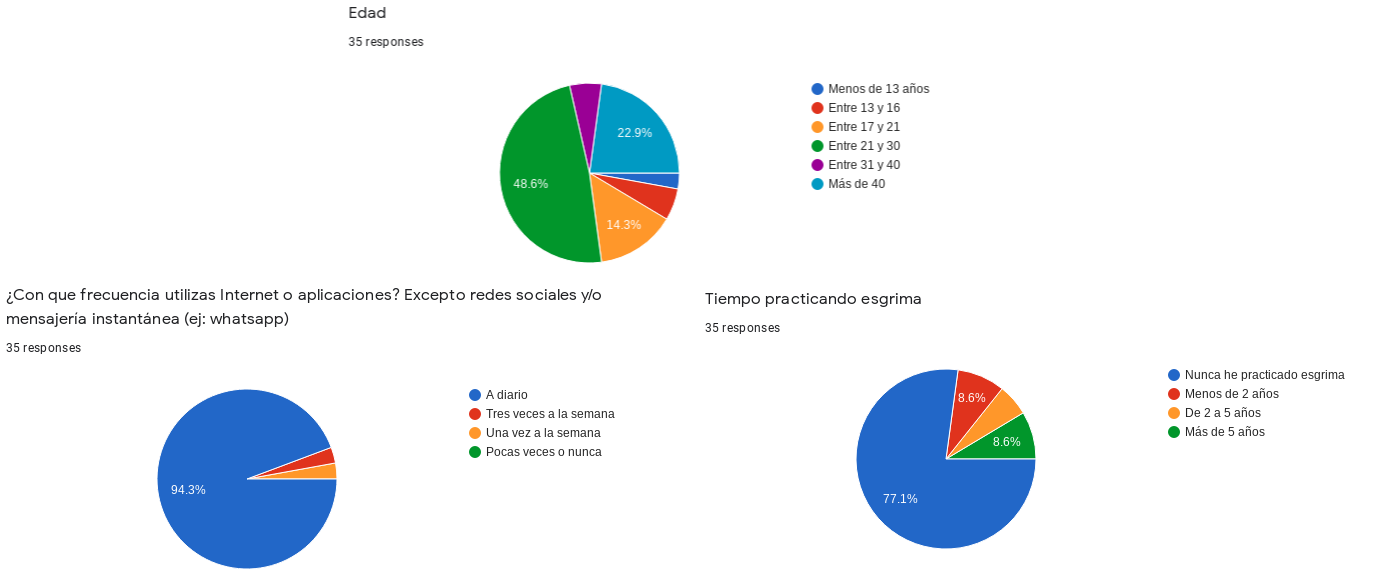
\includegraphics[width=1\linewidth]{respuestas_generales}
	\caption[Características encuestados]{Características encuestados}
	\label{fig:Características encuestados}
\end{figure}

Otra prueba de satisfacción que se llevo a cabo fue una encuesta realizada mediante un formulario
anónimo. Las preguntas formuladas se hicieron con pretensión de conocer cómo de útil les resulto
la herramienta, si la recomendarían y un campo libre para que puedan explicar mejor su opinión.
También se pregunto acerca de los años que se llevaba practicando esgrima, para sacar mas información
acerca del posible conocimiento y público que contestaba a esas preguntas.



Viendo los resultados de la encuesta, se puede descartar la variable de uso de Internet o aplicaciones.
Por otro lado en cuanto a la variable de edad, podríamos discernir tres secciones: menores de 21, entre 21
y 30, más de 30. Respecto a la variable de años haciendo esgrima haremos la diferencia entre aquellos
que nunca hayan practicado esgrima y los que hayan practicado esgrima alguna vez. Siendo esta última
para la evaluación \acl{SUS}.

\subsection{Evaluación interfaz usuario}

Para la evaluación de la interfaz de usuario preguntaremos sobre la claridad a la hora de introducir
los parámetros en los formularios. También se pregunta sobre la ayuda necesaria para completar las preguntas de los formularios.

\subsubsection{Percepción global}

Los resultados de la percepción global global se pueden observar en la \hyperref[fig:Percepción global de interfaz]{figura 5.2}. Se puede apreciar
como las medias son bastante altas por lo que en general, quizás destacando la ayuda necesaria.
Recordemos que 1 es la mejor respuesta. Hay margen de mejora sobre todo en esto último mencionado.
Habrá que reforzar las explicaciones y el feedback.

\begin{figure}[htb]
  \centering
  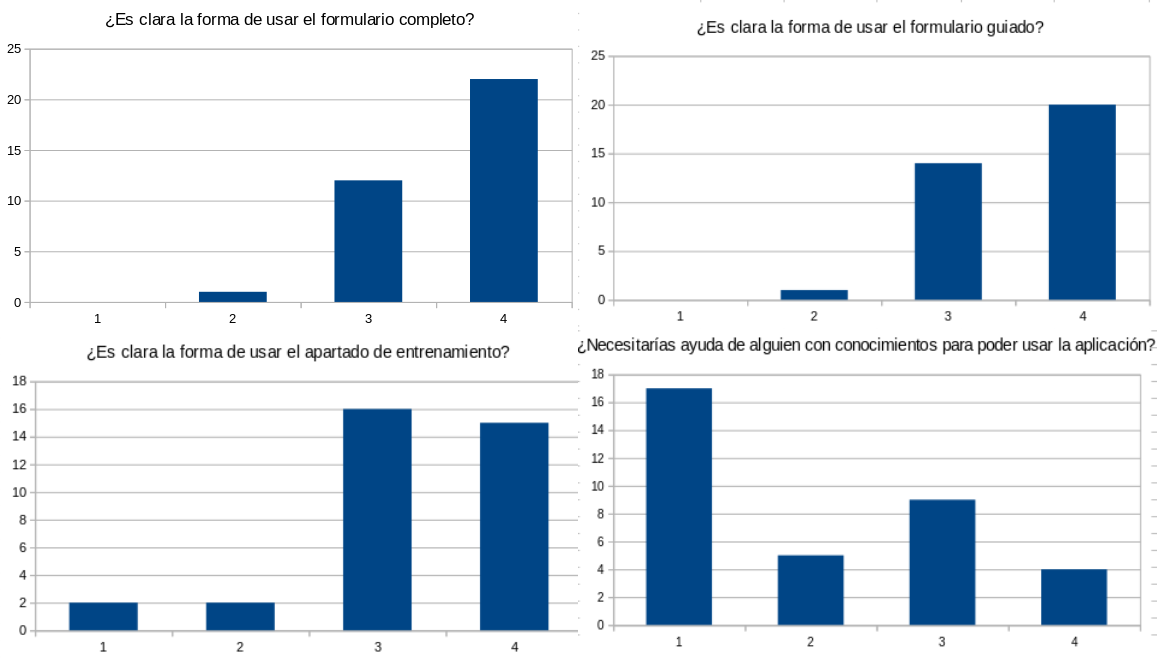
\includegraphics[width=1\linewidth]{interfaz_percepcion_global}
  \caption[Percepción global de interfaz]{Percepción global de interfaz}
  \label{fig:Percepción global de interfaz}
\end{figure}

\subsubsection{Percepción menores de 21 años}

El número de encuestados en este rango fue de 7 personas.

Los resultados de la percepción en menores de 21 años se pueden observar en la \hyperref[fig:Percepción menores de 21 años de interfaz]{figura 5.3}.
Este es el sector que peor ha puntuado el sistema. Habría que destacar la dificultad
que tienen estos mismos para usar el sistema, necesitando ayuda externa.

\begin{figure}[htb]
  \centering
  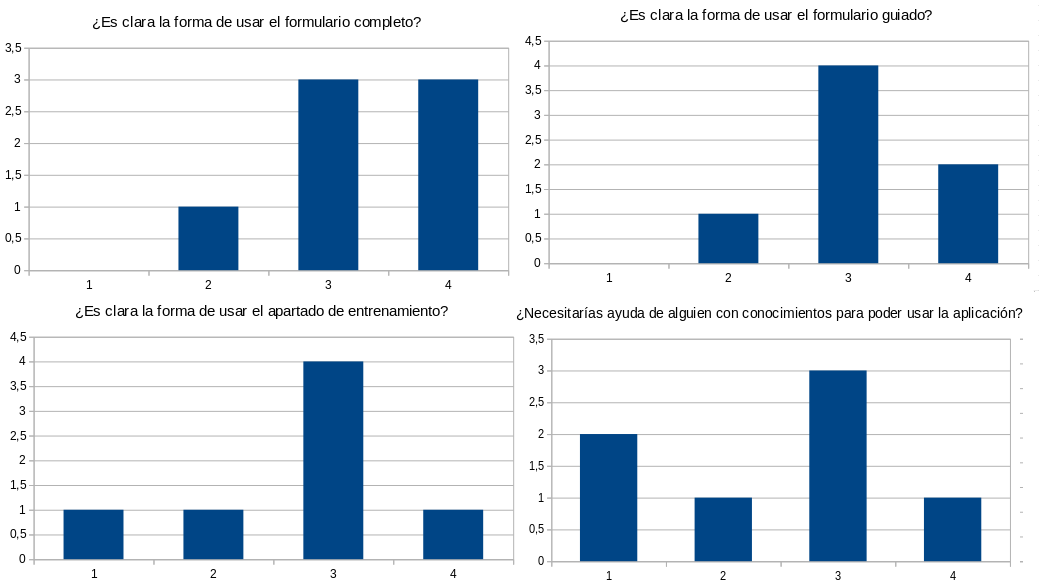
\includegraphics[width=1\linewidth]{interfaz_percepcion_m21}
  \caption[Percepción menores de 21 años de interfaz]{Percepción menores de 21 años de interfaz}
  \label{fig:Percepción menores de 21 años de interfaz}
\end{figure}

\subsubsection{Percepción entre 21 y 30 años}

El número de encuestados en este rango fue de 17 personas. Al igual que en la general las respuestas
son bastante buenas con medias altas. En este sector se puede destacar como necesitan menos ayuda
para utilizar el sistema. Por otro lado, les parece menos clara la forma de utilizar el sistema
de entrenamiento. Los resultados se pueden ver en la \hyperref[fig:Percepción entre 21 y 30 años de interfaz]{figura 5.4}.

\begin{figure}[htb]
  \centering
  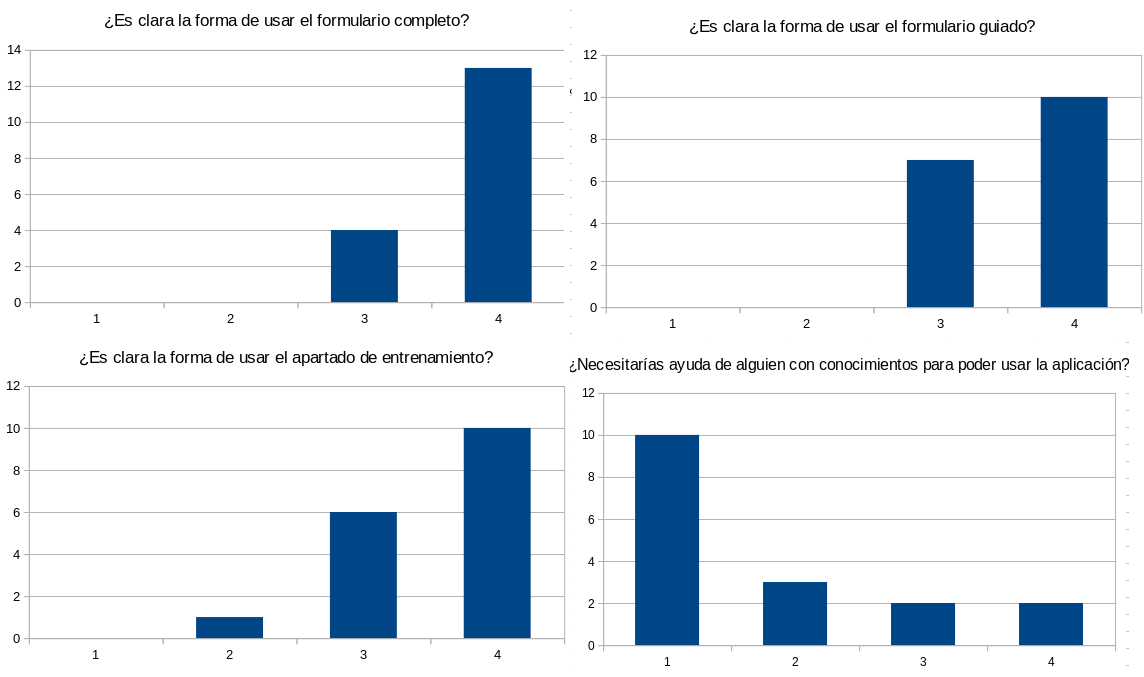
\includegraphics[width=1\linewidth]{interfaz_percepcion_21}
  \caption[Percepción entre 21 y 30 años de interfaz]{Percepción entre 21 y 30 años de interfaz}
  \label{fig:Percepción entre 21 y 30 años de interfaz}
\end{figure}

\subsubsection{Percepción mayores de 30}

El número de encuestados en este rango fue de 10 personas.

Los resultados de la percepción en mayores de 30 años se pueden observar en la \hyperref[fig:Percepción mayores de 30 años de interfaz]{figura 5.5}.
Nuevamente los resultados nos dicen que la aplicación es fácil de usar por las puntuaciones,
siendo estas altas como norma general. Habría que destacar, al igual que en el primer grupo segmentado
han necesitado bastante ayuda para poder usar la aplicación.

\begin{figure}[htb]
  \centering
  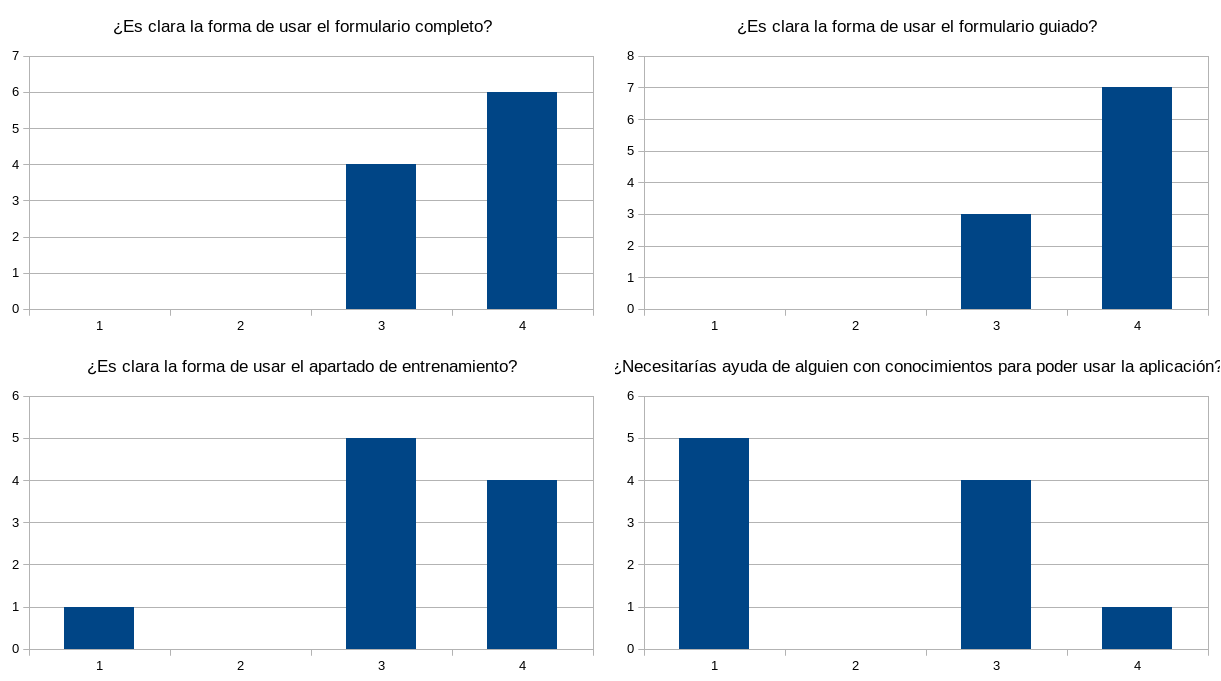
\includegraphics[width=1\linewidth]{interfaz_percepcion_30}
  \caption[Percepción mayores de 30 años de interfaz]{Percepción mayores de 30 años de interfaz}
  \label{fig:Percepción mayores de 30 años de interfaz}
\end{figure}

\subsubsection{Conclusión}
A la vista de los resultados se puede observar como la interfaz de usuario cumple
con las expectativas y es usable en su totalidad. A pesar de los buenos resultados
es apreciable como faltan cosas por mejorar, sobre todo aquellas enfocadas a los
mayores de 30 años y menores de 21. Habrá que hacer foco principalmente en
ayudar a entender las preguntas y respuestas de los formularios. De esta forma
conseguiremos que no haga falta ayuda para usar la aplicación, que fue esta
la parte mas floja.

\subsection{Evaluación \acs{SUS} de la aplicación}
El \acs{SUS}\cite{sus}, es un proceso para la evaluación de éxito
de usabilidad de un objeto, aplicación o sistema en general. Este proceso consiste
en elaborar un cuestionario con 10 preguntas de 4 opciones de respuesta, de este modo
se evitan valores intermedios, forzando al usuario a decantarse por un valor u otro y
normalizando estos después. Este proceso está pensado para cuando no se ha podido
conseguir un gran número de muestras, como es nuestro caso.

\subsubsection{Preguntas}
A continuación se detallan las preguntas a realizar según la base. Estas han sido modificadas
levemente para adaptarse a nuestra aplicación.

\begin{enumerate}
  \item Creo que usaría este [sistema, objeto, dispositivo, aplicación] frecuentemente
  \item Encuentro este [sistema, objeto, dispositivo, aplicación] innecesariamente complejo
  \item Creo que el [sistema, objeto, dispositivo, aplicación] fue fácil de usar
  \item Creo que necesitaría ayuda de una persona con conocimientos técnicos para usar este [sistema,
    objeto, dispositivo, aplicación]
  \item Las funciones de este [sistema, objeto, dispositivo, aplicación] están bien integradas
  \item Creo que el [sistema, objeto, dispositivo, aplicación] es muy inconsistente
  \item Imagino que la mayoría de la gente aprendería a usar este [sistema, objeto, dispositivo, aplicación] en forma muy rápida
  \item Encuentro que el [sistema, objeto, dispositivo, aplicación] es muy difícil de usar
  \item Me siento confiado al usar este [sistema, objeto, dispositivo, aplicación]
  \item Necesité aprender muchas cosas antes de ser capaz de usar este [sistema, objeto, dispositivo, aplicación]
\end{enumerate}

\subsubsection{Medición de resultados}

Para la medición de resultados se deberá seguir el siguiente preproceso:
\begin{itemize}
  \item Invertir las puntuaciones de las preguntas número 10 y 12.
  \item Multiplicar estas puntuaciones por 2,5
\end{itemize}

Una vez hecho el pre-proceso de los datos podremos ver si está por encima
de la media. Para saber si estamos por encima bastará con que el resultado
supere los 68 puntos.

\subsubsection{Puntuación global}
La puntuación fue de 79,75. Esto denota que está muy por encima de la media
por lo que podremos decir que el sistema supera con creces la prueba. A pesar
de esto el resultado denota el amplio margen de mejora.

\subsubsection{Puntuación menores 21 años}
La puntuación obtenida fue de 78. Siendo el segundo público que usará la aplicación
el resultado, a pesar de ser mejorable, es bueno.

\subsubsection{Puntuación entre 21 y 30 años}
La puntuación obtenida fue de 84,2. Público principal por edad y en el que mayor
puntuación se obtuvo superando con creces la media. Siempre es posible mejorar
ciertas partes, pero este no será el foco de mejoras.

\subsubsection{Puntuación mayores 30 años}
La puntuación obtenida fue de 74. Público donde peor puntuación se obtuvo.
Lo ideal sería repetir dicha encuesta haciendo modificaciones para
intentar identificar las causas de estas.

\subsubsection{Puntuación sin experiencia en esgrima}
La puntuación obtenida fue de 79. Mayor parte de los usuarios.
Según comentarios habría que mejorar el feedback que da la aplicación
además de hacer un diseño mas atractivo de la misma

\subsubsection{Puntuación con experiencia en esgrima}
La puntuación obtenida fue de 82. Buena puntuación para aquellos
que tienen conocimiento sobre el tema. Nada que añadir.



\section{Pruebas de campo}
También se utilizó en un entorno cercano. Durante la competición del día 30 de Noviembre se llevó
a cabo el primer ranking de la temporada 2019-2020 de menores de la federación de Castilla-La Mancha.
En dicha competición se facilitó el acceso a la herramienta a María Rosa Maestre, tiradora del club
Espadas de Calatrava. En su fase de grupos tenía un varios enfrentamientos complicados que en anteriores
ocasiones le costo resolver, obteniendo una derrota como resultado en la mayoría de ellos. En el día
del torneo usando la herramienta consiguió sorprender a las tiradoras rivales con nuevas tácticas que
antes no había llevado a cabo. Al hablar con ella se veía mas confianza por lo que este también
pudo ser un factor que le llevara a la victoria. El resultado final para la tiradora fue de
un gran tercer puesto, perdiendo en semifinales en un asalto duro físicamente cuyo ritmo no pudo
seguir. Eligió bien las acciones pero la diferencia vino marcado por el físico de ambas tiradoras.
A destacar que fue quien acabó ganando la competición, esto indica que fue una gran rival contra
quien cayó.

\section{Actualización de la planificación del proyecto}
Después de realizar el desarrollo del proyecto no se pudo completar con éxito la planificación
del mismo. Debido a los problemas encontrados en la iteración 5 vimos como se tuvo que añadir
una semana de desarrollo al proyecto, con los sobre costes que ello supuso. En la figura 5.6
se puede observar cuales fueron los tiempos de desarrollo finales.

\begin{figure}[htb]
  \centering
  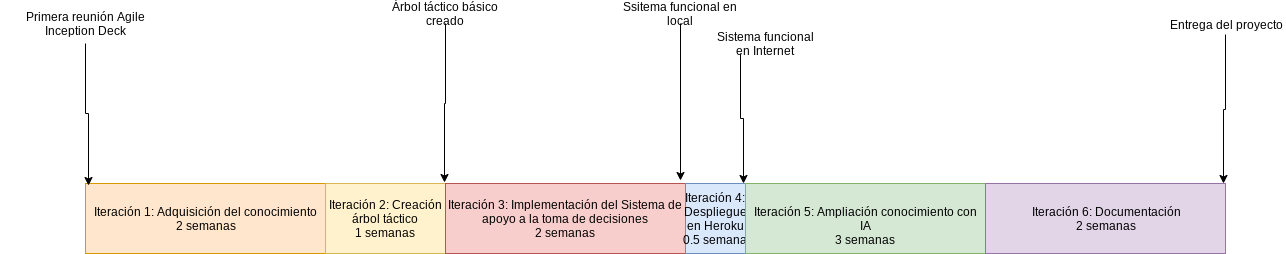
\includegraphics[width=1\linewidth]{LineaTemporalResultados}
  \caption[Características encuestados]{Características encuestados}
  \label{fig:Características encuestados}
\end{figure}

Por suerte, el tiempo extra solo implicó al desarrollador, por lo que no fue el peor de los
casos en cuanto a presupuesto se refiere. Finalmente el coste del proyecto se puede ver en
la \hyperref[tab:costes actualizados del proyecto]{tabla 5.1}.

\begin{longtable}{|c|c|l|l|}
  \caption{Costes actualizados del proyecto}
  \label{tab:costes actualizados del proyecto}

  \endfirsthead
  \endhead

  \hline
  Concepto & Desglose & Horas & Coste \\ \hline
  \multirow{2}{*}{Personal} & Autor del proyecto & 340h & 5440€ \\ \cline{2-4}
  & Experto & 44h & 1320€ \\ \hline
  Infraestructura & Heroku proyect & - & 0€ \\ \hline
  Total & \multicolumn{3}{c|}{6760€} \\ \hline

\end{longtable}
